\textbf{}\documentclass[11pt, a4paper]{report}

% Silbentrennung
\usepackage[ngerman]{babel}

% Umlaute
\usepackage[utf8]{inputenc}

% Pfeile etc.
\usepackage{amsmath}

% Absatz Einrückung 
\setlength{\parindent}{0pt} 

% Silbentrennung
\usepackage[ngerman]{babel}
\usepackage[T1]{fontenc}

% Tabellen
\usepackage{multirow}

%Source Code einfügen
\usepackage{listings}
\usepackage{float}
\usepackage{color}
\usepackage{textcomp}
\lstset{numbers=left, numberstyle=\tiny, numbersep=5pt, tabsize=2,showstringspaces=false, basicstyle=\footnotesize }


% Bibtex
%\usepackage{natbib}
\usepackage{biblatex}
\bibliography{bibliography.bib}
\usepackage{amsrefs}

% Verweise in PDF		
\usepackage{hyperref} 

% Definitionen
\usepackage{amsthm}

\hypersetup{
	colorlinks,
	citecolor=black,
	filecolor=black,
	linkcolor=black,
	urlcolor=black,
	pdftitle={NFC basierte Konfiguration von Lebens- und Arbeitsumgebung},
	pdfauthor={Swen Hutop, Dennis Kluge},
	pdfsubject={Forschungsprojekt},
	pdfproducer={our mac}, % producer of the document
	pdfkeywords={Auto} {Heim} {Automatisierung}, % list of keywords
}

% Glossar
%\usepackage{glossaries}
%\makeglossaries

% für Bilder
\usepackage{graphicx}

% index
%\usepackage{makeidx}
%\makeindex

\begin{document}

\title{NFC basierte Konfiguration von Lebens- und Arbeitsumgebung}
\author{Swen Hutop, Dennis Kluge}

%\pagenumbering{Roman}

% Deckblatte
\thispagestyle{empty}
\begin{center}
\Large{Hochschule für Technik und Wirtschaft Berlin}\\
\end{center}


\begin{center}
\Large{Fachbereich Wirtschaftswissenschaften II}
\end{center}
\begin{verbatim}





\end{verbatim}
\begin{center}
\textbf{\LARGE{Forschungsprojekt 1}}
\end{center}
\begin{verbatim}


\end{verbatim}
\begin{center}
\textbf{im Studiengang Angewandte Informatik}
\end{center}
\begin{verbatim}
















\end{verbatim}

\begin{flushleft}
\begin{tabular}{lll}
\textbf{Thema:} & & NFC basierte Konfiguration von Lebens- und Arbeitsumgebung\\
& & \\
& & \\
& & \\
\textbf{eingereicht von:} & & Swen Hutop  \flq{}swen.hutop@student.htw-berlin.de\frq{}\\
\textbf{eingereicht von:} & & Dennis Kluge  \flq{}dennis.kluge@student.htw-berlin.de\frq{}\\
& & \\
\textbf{eingereicht am:} & & 30. Maärz 2012\\
& & \\
& & \\
\textbf{Betreuer:} & & Herr Prof. Dr. Jürgen Sieck \\
\end{tabular}
\end{flushleft}



% Inhaltsverzeichnis
\tableofcontents


\newpage
%\clearpage\null\vfill


% Abstract
%\begin{abstract}


\end{abstract}

% Alle notwendigen includes

% glossary -  muss als erstes damit die Einträge bekannt sind
%\vfill\null
%\clearpage
\newpage


\chapter{Einleitung}

In Zeiten der digitalen Revolution dringen Gadgets jeglicher Art in die Wohnzimmer, Hosentaschen oder gar Körper von ihren UserInnen vor. So werden moderne Gerätschaften 
nicht mehr als ein Beiwerk zur Unterstützung des Alltags gesehen, sondern fast als ein weiteres Sinnesorgan zur Rezeption der Umwelt interpretiert. 
Jedoch ist bei all dem Drang der Miniaturisierung und des Vordringens in die kleinsten Lebensbereiche ein interessanter Trend zu beobachten. 
Zum größten Teil sind die eigenen Lebensräume von diesem Fortschritt nur mäßig betroffen. In den heutigen Wohnzimmern finden sich zwar Laptops, Flachbildfernseher und viele andere Tools wieder, jedoch ist die eigentliche Infrastruktur bestehend aus Thermostaten, Jalousien usw. wenig betroffen. Die digitale Ansteuerung gestaltet sich als schwer und
kostenintensiv\footnote{Besonders bei der Nachrüstung bestehender Gebäude.}, weiterführende  Konzepte in deren Umgang sind rar gesät. 
\\\\
Besonders bei der Annahme, dass alle 
wichtigen Komponenten eines Haushalts, Büros oder Hotelzimmer digital ansteuerbar sind, ergeben sich interessante Ideen. So sollte die Anpassung der Umgebung nach den eigenen
Bedürfnissen eine Konsequenz sein und in unterschiedlichen Szenarien abspeicherbar. 
Wenn der Gedanke der Konfiguration von Lebensumgebungen mit bereits bestehender und tiefgreifender Infrastruktur weitergeführt wird, ist es leicht auf weitere und 
unterschiedliche Anwendungsszenarien zu blicken. 
So sind beispielsweise Autos ideelle Umgebungen um diese den Wünschen des Fahrer entsprechend zu konfigurieren. Neben Temperatur und Radiosendern können verkehrsrelevante 
Informationen wie etwa die Sitz- und Spiegelpositionen dem Auto bekannt gemacht werden. Als einer der elementaren Frage bleibt offen, in welcher Form die Konfigurationen 
erstellt und verwaltet werden können? Die Antwort liegt buchstäblich in der Hosentasche, so bieten Smartphones die idealen Bedingungen, dank ihrer allgegenwärtigen Präsenz 
und ihres User-Interface.
\\\\
Genau dem eben angerissenen Szenario, möchte sich diese Forschungsarbeit widmen. Derzeit gibt es genau für diese Anwendungsfälle wenig konkrete Lösungen, besonders im 
Umgang und der Übertragung von Konfigurationen. Dabei soll auf eine Vielzahl von unterschiedlichen Lebensumgebungen sei es Autos oder Hotelzimmer eingegangen werden, um 
eine möglichst generisches und skalierbares Prinzip zu konstruieren. 
\\\\
Auf den folgenden Kapiteln wird ausgehend von einer genaueren Skizzierung des aktuellen Stands und der Projektidee, verschiedene Lösungen diskutiert. Neben den Übertragungs- 
und Verteilungswegen, wird ein genauer Augenmerk auf die Gestaltung der Konfiguarationen gelegt. Anschließend sollen die entwickelten Strategien in ein Proof of Concept 
überführt werden. Abschliessend wird ein Fazit über die Ergebnisse dieses Forschungsprojekts gegeben. 
\\\\
Diese Arbeit möchte bewusst eine Vision zeichnen, wie der Umgang mit den vorgestellten Technologien in Zukunft aussehen könnte. In dem hier vorgestellten Umfang sind wenige
Ansätze bekannt, daher wurde sich bewusst dafür entschieden einen möglichst generischen Weg zu gehen. Damit auf den folgenden Seiten nicht stets von \glqq Dem Projekt\grqq 
gesprochen werden muss, wurde sich für den Arbeitstitel \emph{InstantAmbient}\footnote{Basierend darauf, dass die eigene Konfiguration instantan das vorherrschende Ambiente 
ändert. Die Schreibweise im CamelCase orientiert sich an den technischen Aspekt des Projektes.} entschieden.


\chapter{Die Idee von konfigurationsbasierten Systemen}

Dieses Kapitel widmet sich der Gesamtidee von InstantAmbient und diskutiert die Anwendungsszenarien und den Nutzen des Systems. Des Weiteren soll aufgezeigt werden, welche 
Vorteile konfigurationsbasierte Systeme mit sich bringen. 

\section{Die Vision}
Auf die Vision hinter InstantAmbient wurde bereits in der Einführung kurz eingegangen. Es geht darum ein System so zu konzipieren, mit dessen Hilfe es möglich sein soll 
unterschiedlichste Umgebungen nach den eigenen Bedürfnissen anzupassen. Für ein besseres Verständnis soll kurz der Alltag einer fiktionalen Person gezeichnet werden, welche
bereits ausgiebig konfigurationsbasierte Systeme nutzt. 
\\\\
Wir begleiten einen Tag lang Frau Schröter ihres Zeichens Senior Software Developer bei IBM Deutschland und gerade auf Geschäftsreise in London für eine Schulung zur 
Entwicklung mit Ruby on Rails. Sie nutzt seit geringerer Zeit konfigurationsbasierte Systeme und wendet diese so oft wie möglich an. Nach der Ankunft in Haethrow beschließt 
sie der Mobilität wegen sich ein Mietwagen bei dem bekannteren Anbieter RentX zu nehmen. Dieser rüstet seit einiger Zeit eine Vielzahl seiner Fahrzeuge mit 
konfigurationsbasierten Systemen aus. Nachdem das Auto angemietet wurde und Frau Schröter ihre Schlüssel erhielt, brauch sie nur noch einzusteigen und mit Hilfe der 
integrierten NFC-Schnittstelle\footnote{Welche genau in Frage kommen, ist Teil der Fragestellung.} des Automobils ihre persönliche Konfiguration mit dem Smartphone und einer 
passenden App überspielen. Da sie bereits mehrere Male mit einem Wagen gleichen Typs gefahren ist, war eine passende Konfiguration vorhanden. So stellt sich vollautomatisch
neben den Außenspiegeln der Sitz auf die korrekte Position ein und im Autoradio läuft der präferierte Musikstream von Frau Schröter mit entspannenden Jazzklängen. Natürlich
stellt sich die Klimaautomatik auf eine mollige Temperatur von 21°C ein. Perfekte Umstände für eine sichere Fahrt zum Hotel.
\\\\
Standesgemäß wurde das Hotelzimmer bereits Online gebucht und bezahlt. Als Zugangsschlüssel wurde ein Key generiert, welcher in eine bestehende oder neue Konfiguration 
eingebettet werden kann. So ist der unter Umständen lästige Check-In etwa durch Zeitdruck nicht mehr notwendig. Das Zimmer muss nur noch bezogen werden. Da Frau Schröter das
erste mal Kundin bei dieser Hotelkette ist, hat sie bereits während des Fluges eine Konfiguration für das Zimmer angelegt und den Key zugewiesen. Hierfür musste Sie jedoch 
nicht komplett ihre persönlichen Vorlieben nochmals eingeben, sondern konnte bestehende Profile anpassen. Der Schliessvorgang und die Übertragung der Konfiguration kann so 
innerhalb eines kurzen Knopfdruckes geschehen. Frau Schröter ist dank der Londoner Rush-Hour spät dran und hat lediglich Zeit ihre Koffer abzustellen um anschließend gleich
zum Schulungsort weiterzufahren. Auf dem Weg in die Tiefgarage ändert sie die Innentemperatur auf 19°C, da es ihr vorhin im Auto zu warm war. 
\\\\
Am Schulungsort angekommen, erhält jede/r TeilnehmerIn einen Schreibtisch zugewiesen um das gelernte Wissen sofort anwenden zu können. Die Schreibtische sind Prototypen der
Firma InstantDesk und bieten ebenfalls die individuelle Konfiguration. Wie es der Zufall will, hat Frau Schröter bereits ebenfalls seit einigen Wochen einen Tisch gleichen
Typs für Beta-Tests in ihrem Büro. Nachdem die Konfiguration aktiviert wurde, sind Tischhöhe, Verbindungen zum VPN-Netzwerk über den integrierten Router und andere 
Belange automatisch eingestellt. Dies sorgt für einen gelungenen Einstieg in die Schulung. 
\\\\
Nach einem langen Arbeitstag kehrt Frau Schröter zurück in ihr Hotelzimmer, dass bereits bei Ankunft ihren Lieblingsfilm geladen hat. Während sie auf der Couch ein Glas Wein 
genießt, ändert sie die Lichteinstellungen im Schlafzimmer und lässt sich ein Bad ein. 
\\\\
Zugegeben ist die hier gezeigte Vision sehr idealisiert dargestellt. Sie soll aber zeigen in welchen Umfang konfigurationsbasierte Systeme eingesetzt werden können. So sind 
wie gezeigt unterschiedlichste Szenerien vorstellbar, welche sich durchaus miteinander kombinieren lassen. Die kleine Geschichte rund um Frau Schröter soll einen Einblick und 
ein Verständnis dafür liefern, in welcher Art und Weise diese Systeme agieren können.  
Um es vorweg zu nehmen derzeit gibt es kein einziges System, welches diese Aufgaben erfüllen kann. Auch ist es möglich einen ersten Einblick in die mögliche 
Komplexität\footnote{Eine der Zentralfragen.} einer generischen Antwort zu zeigen. 
Teile der Vision werden im Laufe dieser Arbeit extrahiert, und zu einem eigenen Lösungsmöglichkeit zusammengefügt. Am Ende soll ein Proof of Conecpt den Entwurf validieren. 

\section{Warum konfigurationsbasierte Systeme?}
Im letzten Abschnitt wurden bereits unterschiedlichste Anwendungsszenarien aufgezeigt. Natürlich lässt sich provokant die Frage stellen warum überhaupt konfigurationsbasierte
Systeme angebracht sind. Um nicht zu viel dem 3. Kapitel vorwegzunehmen sind derzeit nur wenige Umgebungen konfigurierbar, was an unterschiedlichen Gründen 
liegt\footnote{Mehr dazu im nächsten Kapitel.}.
\\\\
Eine Untermenge der Vorteile lassen sich dennoch bereits aus der Vision herauslesen neben der Befriedigung der eigenen Bedürfnisse, haben besonders die Anbieter solcher 
Umgebungen Vorteile. So ist dem Autovermieter RentX daran gelegen, dass seine Kunden so sicher wie möglich das Auto bewegen um das Risiko auf Schäden zu minimieren. Die 
FahrerInnen finden stets ihre Konfiguration vor, welche in den meisten Fällen durch andere Fahrten erprobt ist.
\\\\
Hotelketten können einen besonderen Service anbieten. Neben der individuellen Gestaltung der Zimmer, ist es möglich Vorgänge wie Check-Ins zu vermeiden und die Schlüssel 
bereits vorab zu übertragen. Bei weiterer Betrachtung ist es sogar möglich zu sagen, dass die Bedienung von Multimedia-Geräten nichts anderes als eine Änderung der aktuellen
Konfiguration ist. Die Wege welche hier bestritten werden können, sind durchaus vielseitig. 
\\\\
Zu guter Letzt ist es möglich auch exotischere Beispiele zu finden wie etwa die Konfiguration von Schreibtischen und den damit verbundenen Netzwerken zu ermöglichen. 
Die Möglichkeiten können bis zum Intelligenten Energiemanagement und darüber hinaus gehen.
Warum ein Forschungsbemühen in diese Richtung angebracht ist, liegt auf der Hand. So können eine Vielzahl an Parteien einen praktischen Nutzen durch die Anwendung von 
konfigurationsbasierten Systemen ziehen.

\section{Gewählte Ansätze von InstantAmbient}
Innerhalb der Projektarbeit ist es alleine aus zeitlichen Gründen die Behandlung aller einzelnen Teilaspekte nicht durchführbar. So wird sich innerhalb der nächsten Kapitel 
speziell auf die Teilbereiche der Automobile und Hotelzimmer gestützt, jedoch immer mit dem Anspruch eine generischen Ansatz zu produzieren, welcher sich auf neue 
Anwendungsgebiete ausweiten lässt. Im besonderen Hauptaugenmerk liegt der Aufbau und die Gestaltung von Konfigurationsdateien, wobei eine Vielzahl von unterschiedlichen 
Mechanismen berücksichtigt werden, sowie die Konzipierung der App und Backenddienste\footnote{Damit sind all die Dienste gemeint, welche die Konfigurationen entgegen nehmen 
und weiterverarbeiten.}. Im Fokus stehen die Probleme der Informations- und Datenverarbeitung, weiterführende Überlegungen wie etwa zu Geschäftsmodellen werden nicht 
angestellt. 
\\\\
Das nächste Kapitel widmet sich zunächst der Betrachtung bestehender Lösungen um anschließend vollendsw die Lösungsstrategie von InstantAbient aufzuzeigen. Hierfür wird 
zunächst die Gestaltung von Konfigurationen diskutiert um anschließend die datenverarbeitenden Mechanismen zu konstruieren. 


\chapter{Bekannte Lösungen}
Das macht Swen :) 

\section{Gegenwärtiger Stand}
\subsection{Allgemeine Situation}
\subsection{Bekannte Lösungen}
\subsection{Aufzeigbare Probleme}
- wo sind aktuelle Probleme?

- unbedingt recherche betreiben 
- was haben wir da, gibt es überhaupt etwas? 

% Konfiguration
\chapter{Konfigurationen}

\section{Definition einer Konfiguaration}
- wie definiert sich eine konfiguration, was ist sie
- Aufbau einer Konfiguration

\section{Aufbau}
\section{Datenformate}
-XML
-YAML
-JSON 

Entscheidung auf JSON vergleich der Dateoigrößen anführen.




\section{Priorisierung}
\section{Vorhersage}
\section{Echtzeit-Änderungen}

% Loesungen
\chapter{Lösungsansatz}
% Architektur und Technologien
\chapter{Die Architektur}
% Client
\chapter{Der Client}
Dieses Kapitel beschäftigt sich mit dem Smartphone-Client, der den Projektnamen AmbientClient trägt. Hierbei wird auf die Konzipierung des Clients sowie den Ablauf einer anzulegenden Umgebung und das Senden dieser eingegangen. 

\section{Konzipierung und Entwicklung der Benutzeroberfläche}
Nach der Festlegung der Lösungsstrategie, die InstantAmbient verfolg, musste ein Bedienkonzept für die App erarbeitet werden. Diese soll, wie schon mehrfach angesprochen wurde, schnell verständlich und kurze Bedienwege für den Benutzer bereitstellen. \\ 
Wie im Kapitel der Konfigurationen bereits angesprochen gibt es Sektionen. Da InstantAmbient sowohl für Autos als auch für Hotels funktionieren soll, wurde eine Allgemeine Konfiguration die elementare Möglichkeiten enthält konstruiert. Da diese sozusagen als Globale Konfiguration dienen, werden sie mit dem Start der Anwendung abgefragt. Dies gibt den/der BenutzerIn die Möglichkeit von vornherein die ersten Einstellungen vorzunehmen und auf seinem Gerät zu speichern.  

\begin{figure}[H]
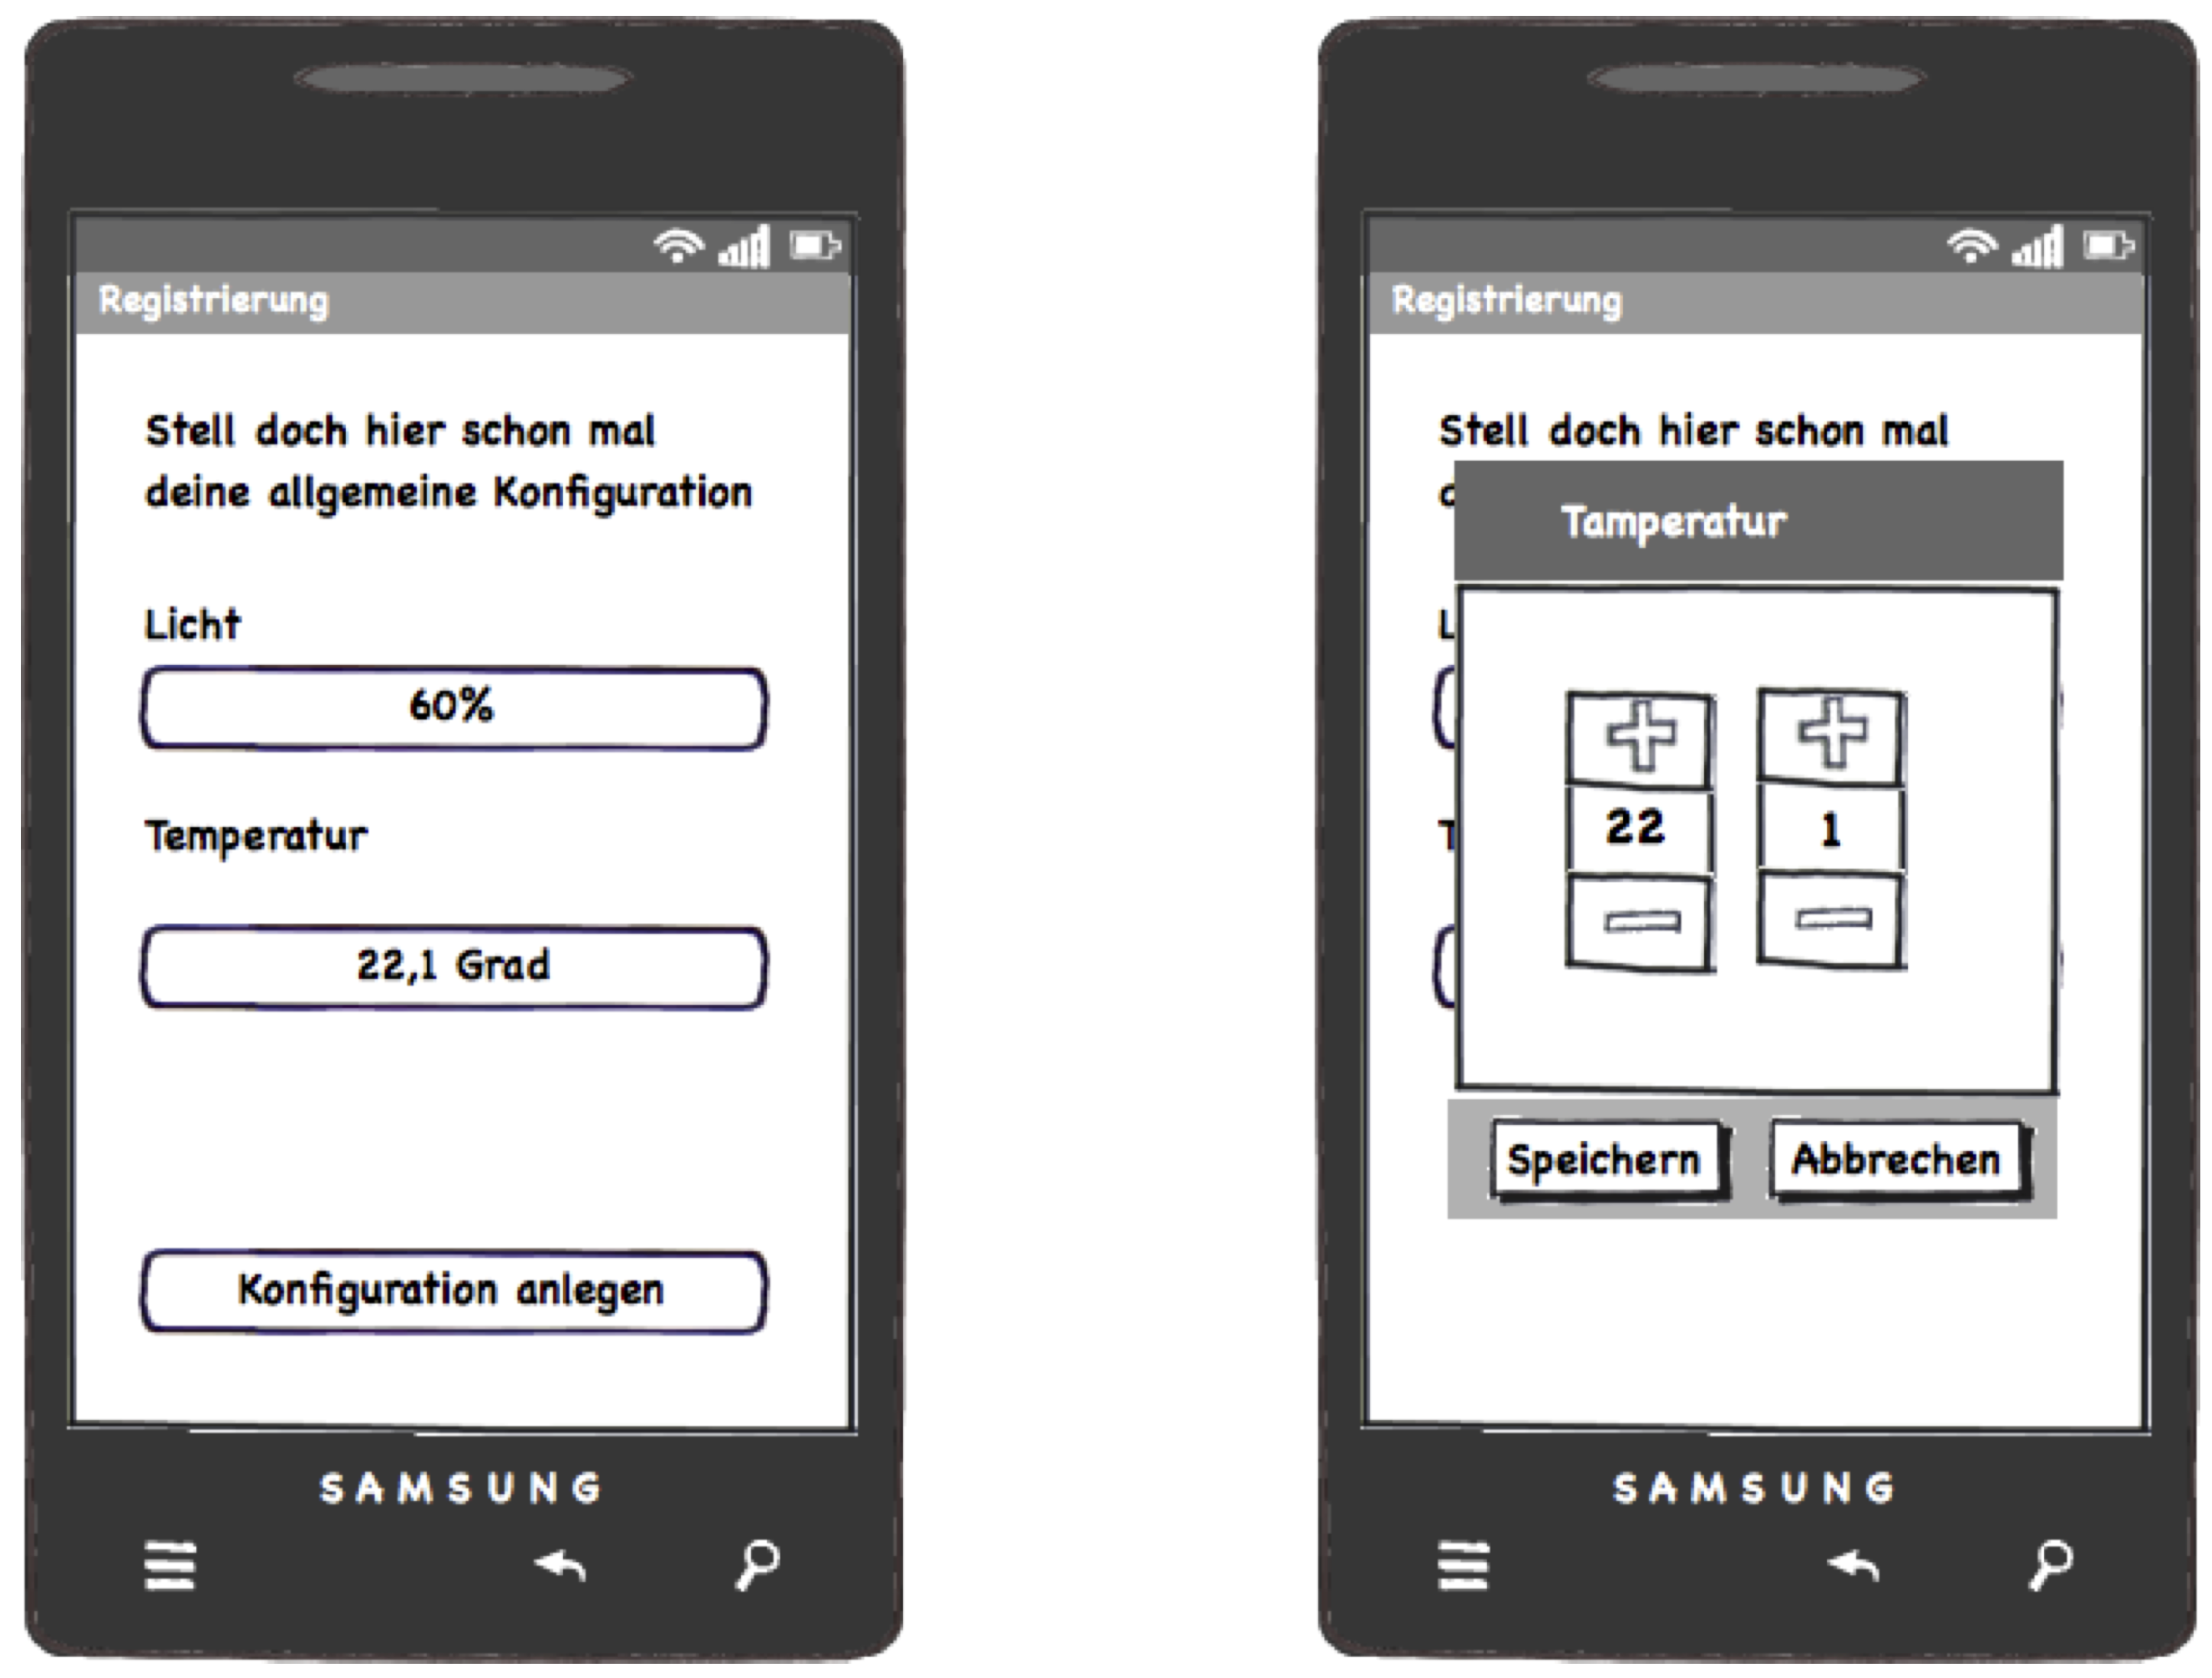
\includegraphics[width=12.5cm]{MockUps/Registrierung}
\caption{MockUp der Registrierung}
\end{figure}

Nachdem der/die BenutzerIn diese angelegt hat, wird er/sie in die Umgebungsübersicht geführt. Hier sieht er/sie alle von ihm/ihr angelegten Umgebungen. Durch das Anklicken dieser kommt er/sie auf die Detailseite der Umgebung und kann diese gegebenenfalls ändern.       
Des Weiteren hat er/sie die Möglichkeit in der Übersicht im Menü eine neue Umgebung anzulegen oder die Allgemeine Konfiguration zu ändern. Dadurch ist diese von den Umgebungen getrennt veränderbar. Allerdings haben die Benutzer die Möglichkeit die Allgemeinen Konfigurationsdaten für eine Spezifische Umgebung zu ändern ohne die allgemeine Konfiguration zu verändern. 

\begin{figure}[H]
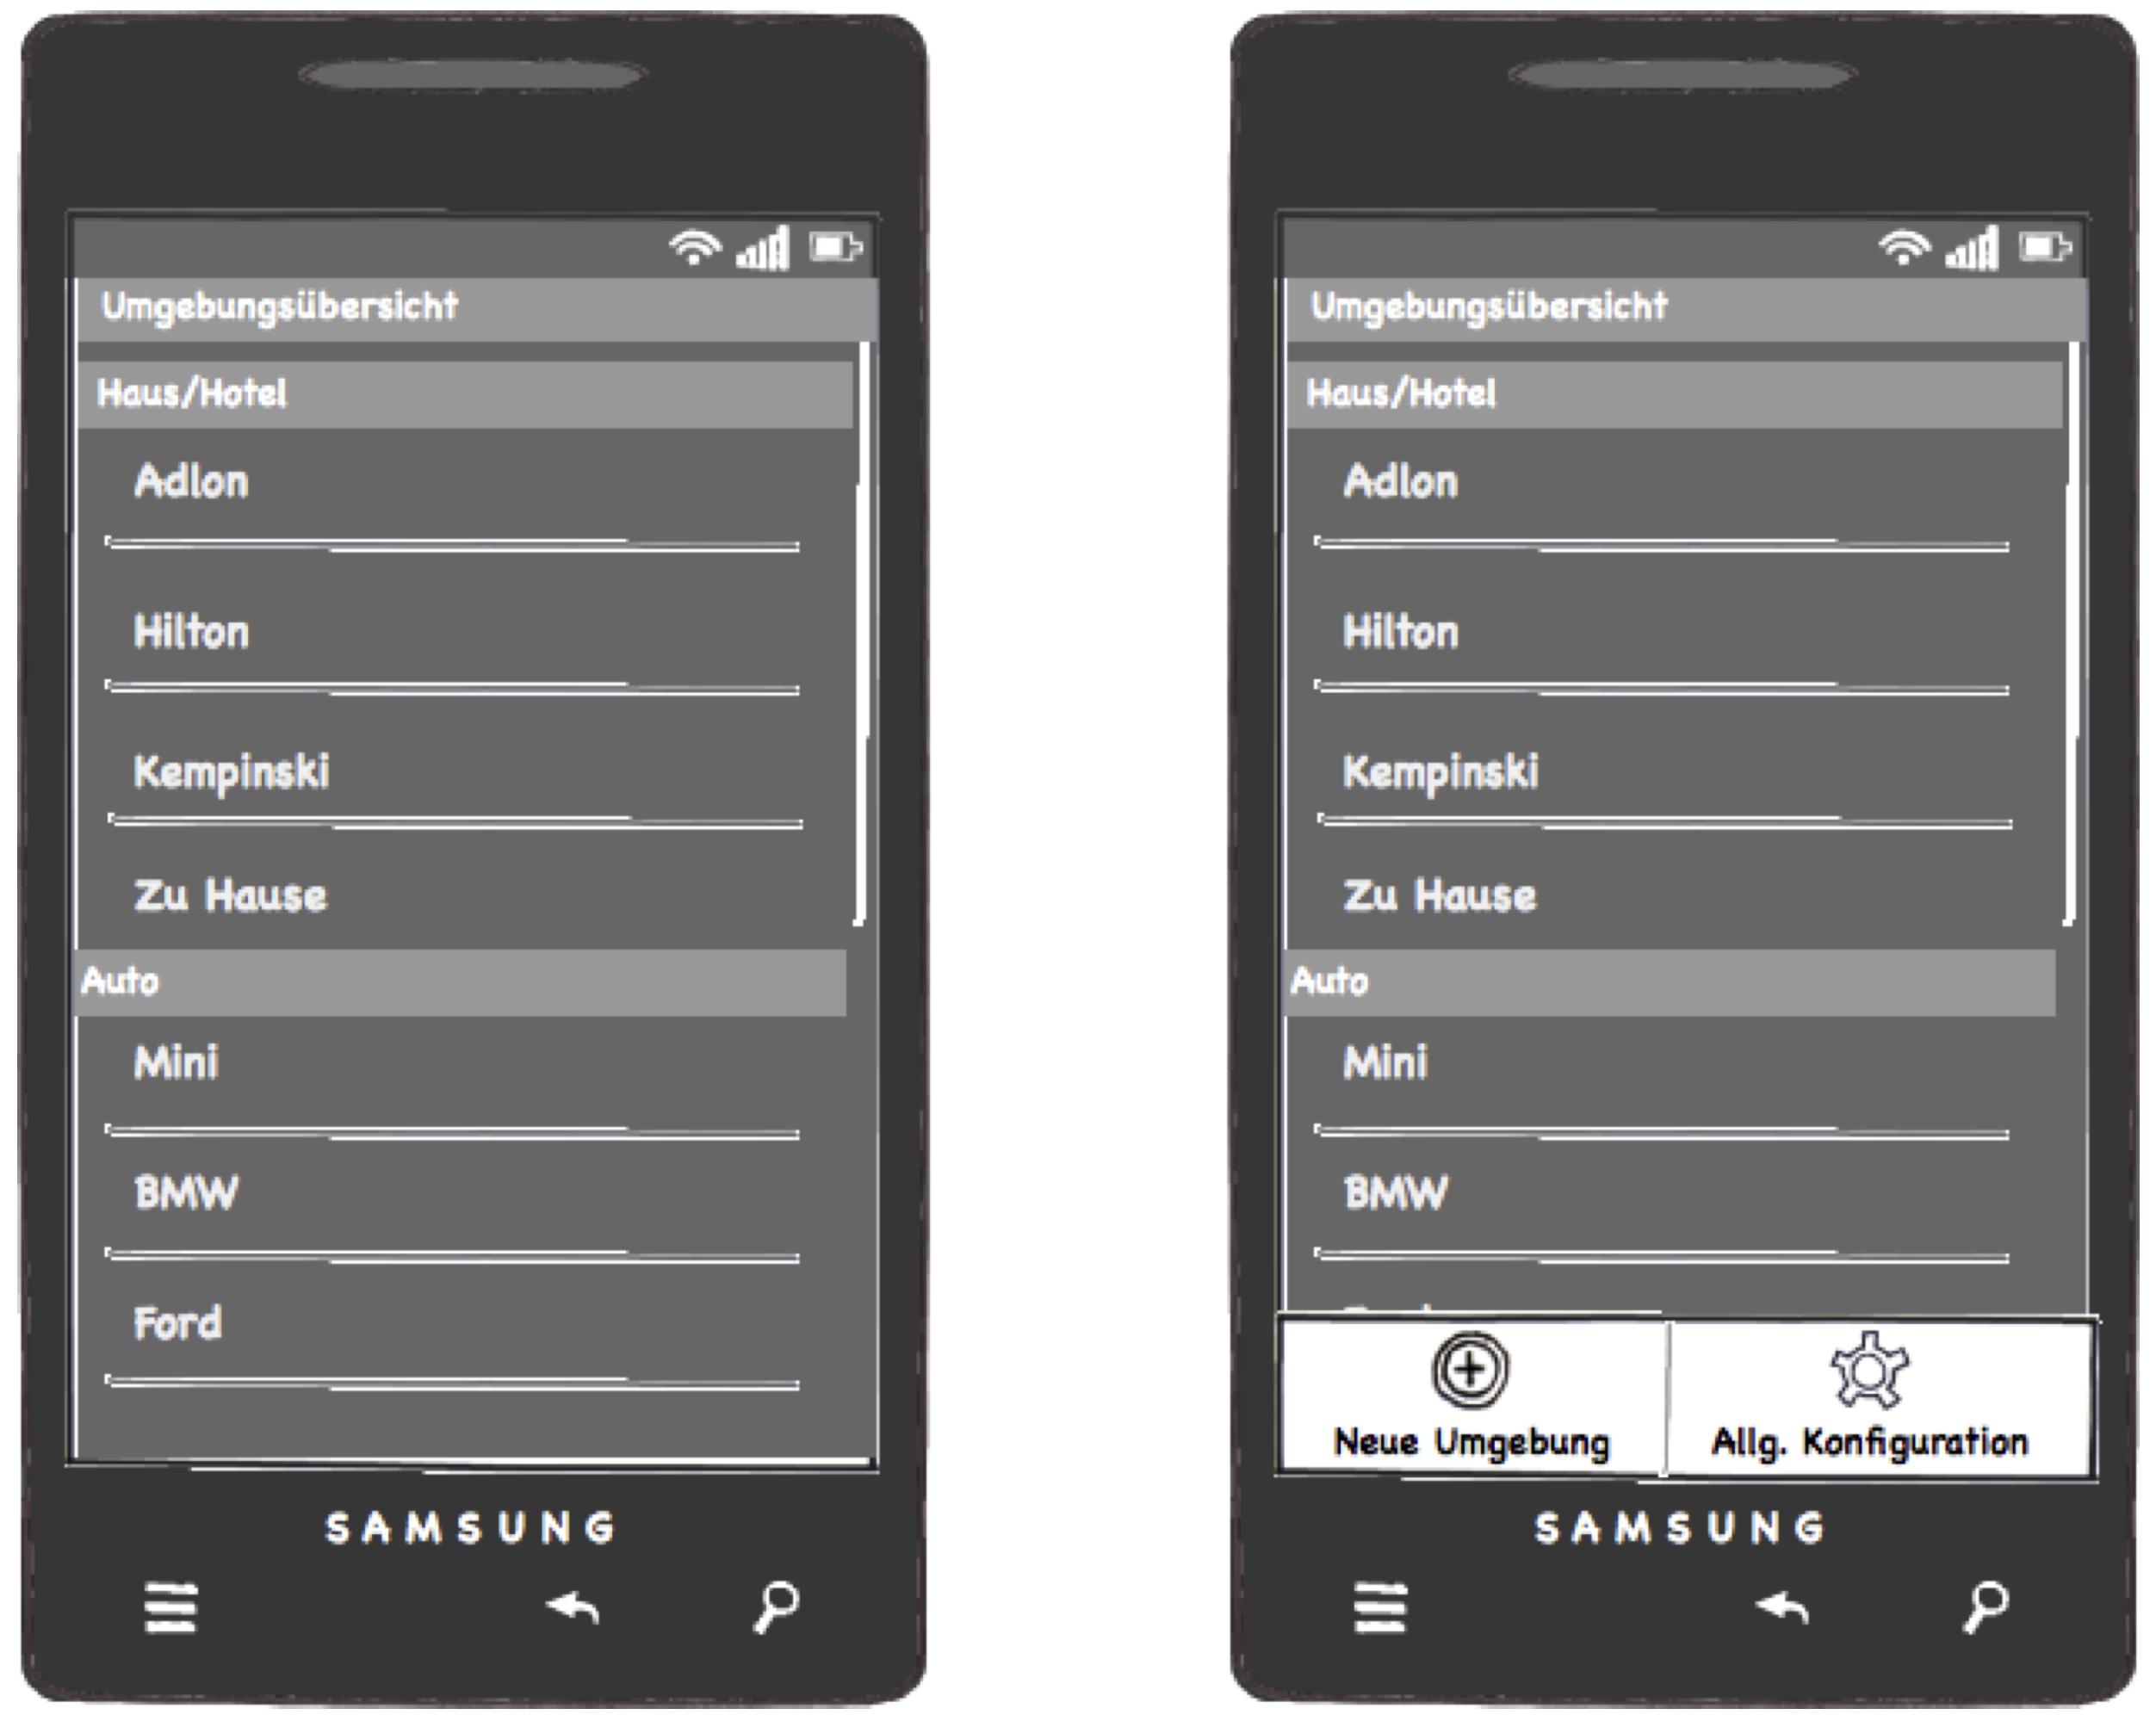
\includegraphics[width=12.5cm]{MockUps/Umgebung}
\caption{MockUp der Umgebungsübersicht}
\end{figure}

Es gibt also drei verschiedene Hauptansichten. Die Umgebungsübersicht, die Umgebungsansicht und die Ansicht für die Allgemeine Konfiguration. Die Anwendung wurde sehr schlicht gehalten und nicht mit Auffälligen optischen Spielereien bestückt. Die Oberfläche soll die Benutzer nicht ablenken, sondern den Fokus auf die Einstellungen legen. 
\\\\
Des Weiteren wurde auch eine mögliche Konzeption entwickelt wenn sich ein/e BenutzerIn zum zweiten mal in einem Hotel befindet, nur das dieses mal die Ausstattung des Zimmers mehr Möglichkeiten bietet. Hierbei sollte das Backend den Client über die neuen Möglichkeiten informieren und dieser meldet dies dem/der BenutzerIn und gibt ihm/ihr hierbei gleich die Möglichkeit ein neues Profil für die Umgebung anzulegen. Dieses Konzept ist aber nicht in der Anwendung umgesetzt worden. Da hierbei das Ziel war eine einfache Konfiguration zu erstellen und zu Übertragen.

\begin{figure}[H]
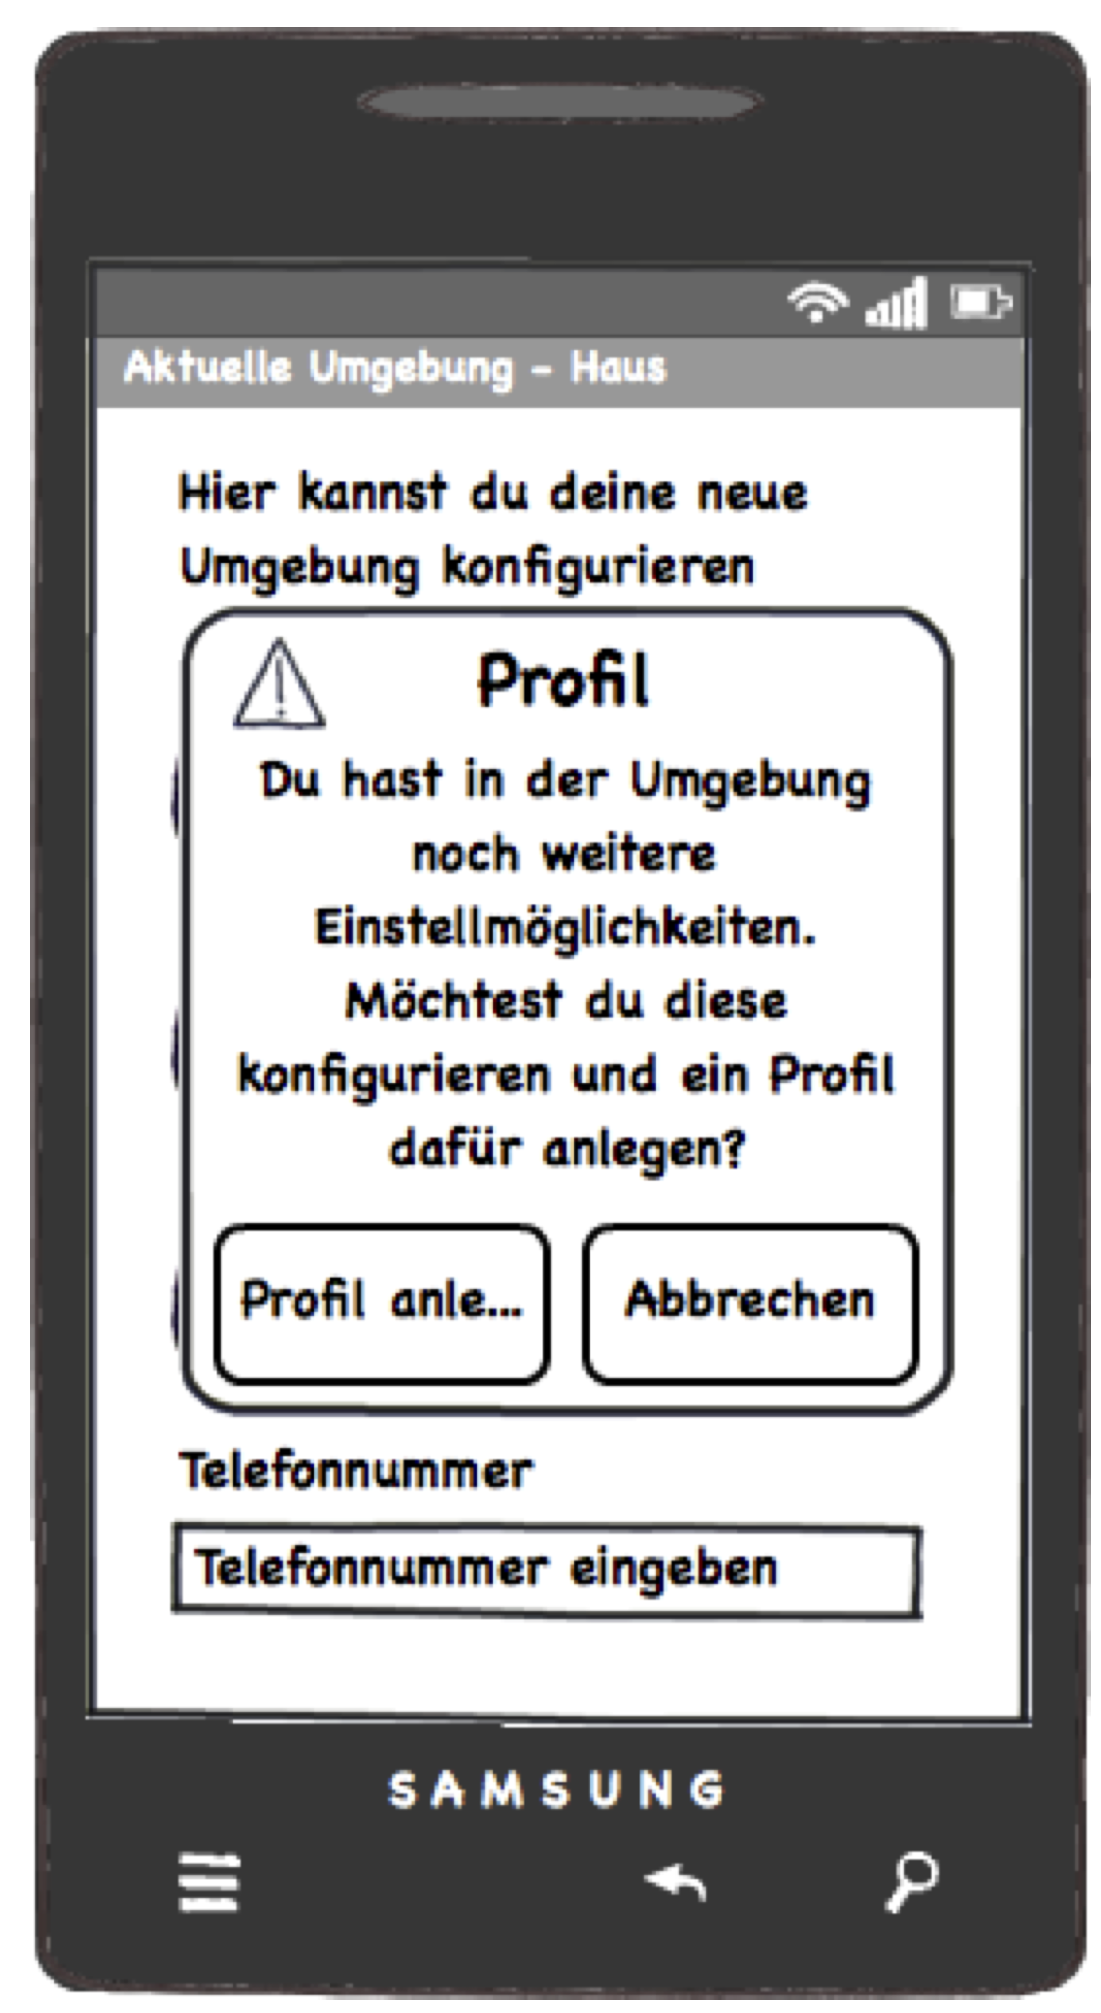
\includegraphics[width=6cm]{MockUps/Erweiterung}
\caption{MockUp der Profilerweiterung}
\end{figure}

\section{Umsetzung} 
Nach dem die Konzeption und die Benutzerführung anhand der Mock-Ups stand, wurde die Anwendung entwickelt. Bei der Verwendung des SDK wurde auf die letzte verbreitete Smartphone Version von Android zurückgegriefen. Damit die Konfiguration vom Licht oder von der Temperatur eingestellt werden kann wurde ein NumberPicker verwendet. Dies führte ein Problem mit sich, auf das im Abschnitt Probleme eingegangen wird. Als Datenbank wurde die von Android bereitgestellte SQLite Datenbank verwendet. Ein wichtiger Bestandteil neben der Oberfläche ist die Bluetoothschnittstelle. \\
Diese wurde als Service implementiert und kann somit unabhängig von der Anwendung im Hintergrund laufen. Dies ist ein wichtiger Punkt vom AmbientClient, da der Benutzer möglichst wenig mit dem starten des Übertragungablauf zu tun haben soll. Zumindest soll es für den Benutzer nicht offensichtlich sein. In dem Prototypen wird der Service mit dem öffnen der Anwendung, in der Umgebungsübersicht gestartet. Damit die Anwendung Bluetooth verwenden kann muss dieses zu aller erst eingeschalten werden. Dies wird beim Ersten Start, nachdem die Allgemeine Konfiguration angelegt wurde, abgefragt und der Benutzer wird gegebenenfalls darum gebeten dieses einzuschalten. Der Service kann jederzeit erweitern und verändert werden. Dies ist ein Grund warum diese Schnittstelle als Service aufgebaut wurde. Hierbei muss dieser aber den Namen der Einheit kennen mit der er sich verbinden soll, bevor er mit diesem ein Pairing durchführen kann. Sobald der Client etwas gefunden hat beginnt er eine Verbindung aufzubauen, die Daten aus der Datenbank zu laden und als JSON Objekt an den Connector zu senden. Da dies völlig automatisch im Hintergrund passiert, erhält der Benutzer keine Rückmeldung falls die Übertragung erfolgreich war.

\section{Probleme}

Ein Problem was sich bei Android als immer wiederkehrend zeigt ist, dass bei der Konzeption von Android einige Fehler gemacht wurden. Zum Beispiel ist es möglich den in der Anwendung verwendete NumberPicker in der Grafischen Oberfläche einzubauen, doch kann man diesen nicht im Code einbinden, da er erst ab dem API Level 11, welches auch als Android 3.0 bezeichnet wird, zur offenen Verfügung steht. Diese Android Version ist allerdings nur für Tablets. Aus diesem Grund mussten extra zwei Klassen die den NumberPicker bilden eingebunden werden. Es ist ein typisches Androidphänomen, dass gewisse Möglichkeiten erst in späteren Versionen bereitgestellt werden, obwohl der Ansatz schon seit API Level eins vorhanden ist. Ein weiteres Problem bei Android sind die verschiedenen Benutzeranischten. Jede Anwendung verfolgt ihren eigenen Weg. Es entsteht keine Einheitliche Struktur. Der einzigen Struktur zur Navigation ist das Menü welches mittels Taste aufgerufen werden kann und die Zurücktaste, die einen gegebenenfalls in die letzte Ansicht zurückbringt oder die App schließt.  


\section{Zusammenfassung Client}

Dieser Abschnitt sollte einen überblick über das gewählte Konzept, die Benutzerführung sowie die für den Prototypen Umgesetzten Funktionen geben. Im nächsten Abschnitt folgt die Umsetzung des Backend.  



% Backend
\chapter{Das Backend}

\section{Anforderungen}
\section{InstantConnector}
\section{InstantBrain}
\section{InstantActor}

% Ausblick und Zusammenfassung
\chapter{Ausblick}
\newpage


% Abbildungsverzeichnis
\listoffigures
\addcontentsline{toc}{chapter}{Abbildungsverzeichnis}

%Code-Verzeichnis
\renewcommand{\lstlistlistingname}{Verzeichnis der Quelltextauszüge}
\lstlistoflistings
\addcontentsline{toc}{chapter}{Verzeichnis der Quelltextauszüge}

% Bibtex mit der externen Datei bibliography.bib
\nocite{*}
\printbibliography
\addcontentsline{toc}{chapter}{Literaturverzeichnis}

\end{document}
